\documentclass[10pt,twocolumn,letterpaper]{article}

\usepackage{cvpr}
\usepackage{times}
\usepackage{epsfig}
\usepackage{graphicx}
\usepackage{amsmath}
\usepackage{amssymb}
\usepackage{kotex}

% Include other packages here, before hyperref.

% If you comment hyperref and then uncomment it, you should delete
% egpaper.aux before re-running latex.  (Or just hit 'q' on the first latex
% run, let it finish, and you should be clear).
\usepackage[breaklinks=true,bookmarks=false]{hyperref}

\cvprfinalcopy % *** Uncomment this line for the final submission

\def\cvprPaperID{****} % *** Enter the CVPR Paper ID here
\def\httilde{\mbox{\tt\raisebox{-.5ex}{\symbol{126}}}}

% Pages are numbered in submission mode, and unnumbered in camera-ready
%\ifcvprfinal\pagestyle{empty}\fi
\setcounter{page}{1}
\begin{document}

%%%%%%%%% TITLE
\title{PROJECT2. Human Action Recognition using Hidden Markov Model}

\author{Sangjun Son\\
Seoul National University\\
Department of Computer Science and Engineering\\
{\tt\small lucetre@snu.ac.kr}
}

\maketitle

\section{Introduction}

Hidden Markov Model has such a good strength in analysing sequential data, and had been widely used in language model, part-of-speech tagging and named entity recognition \cite{ratgo}. Based on Markov process, HMM infers probability distributions of the model from observations and find the most likely results so far. It is useful for cases unable to observe all datasets and only able to get its causal evidences, and can be applied in many different data restoring fields \cite{hmmwiki}, e.g. multiple DNA sequence alignment, protein secondary structure prediction \cite{biology} and speech recognition. Datasets being used in HMM modelling should be time-serial. For example, speech recognition has temporal structure consisted of statistical models and can be encoded as a sequence of spectral vectors spanning the audio frequency range \cite{speechrecognition}.

Likewise, we'd like to use temporal human action sensor data to make Human Action Recognition system (HAR) using HMM. We've trained our model with  Human Activities and Postural Transitions datasets (HAPT) produced by Jorge L, \etal \cite{hapt}. Measurement was done by 30 volunteers carrying a waist-mounted smart phone with embedded inertial sensors. Dataset includes 61 experiments with 30 participants and measured in 50Hz frequency and about 400s duration per experiment. Each experiment contains 12 types of human actions like standing, walking down, \etc. We separated into 12 part of data so we can easily train our model by action type. Eventually, we've got 1,214 examples and randomly split as train and test dataset as 9:1 ratio respectively.

%-------------------------------------------------------------------------
\section{Related Works}
Human activity recognition is nowadays an active research field which aims to understand human behaviour and there have been lots of researches to figure out human behaviours. One of the approaches was method consisted of support vector machines (SVMs) and temporal filters of activity probability estimations within a limited time window \cite{haptpaper}. Probability estimation after feature extraction was done by MAP filtering.

Rubén San-Segundo, \etal have implemented system comprising of three main modules: feature extraction, HMMs training and activity recognition. In the training module, 6 HMM modules were being trained to classify human actions with datasets of only six different physical activity types: walking, walking-upstairs, walking-downstairs, sitting, standing and lying down. Due to the lack amount of activity types they've obtained the recognition error rate of 2.5\% \cite{monitoring}.

%-------------------------------------------------------------------------
\section{Preliminaries}

\subsection{Hidden Markov Model}

\begin{center}
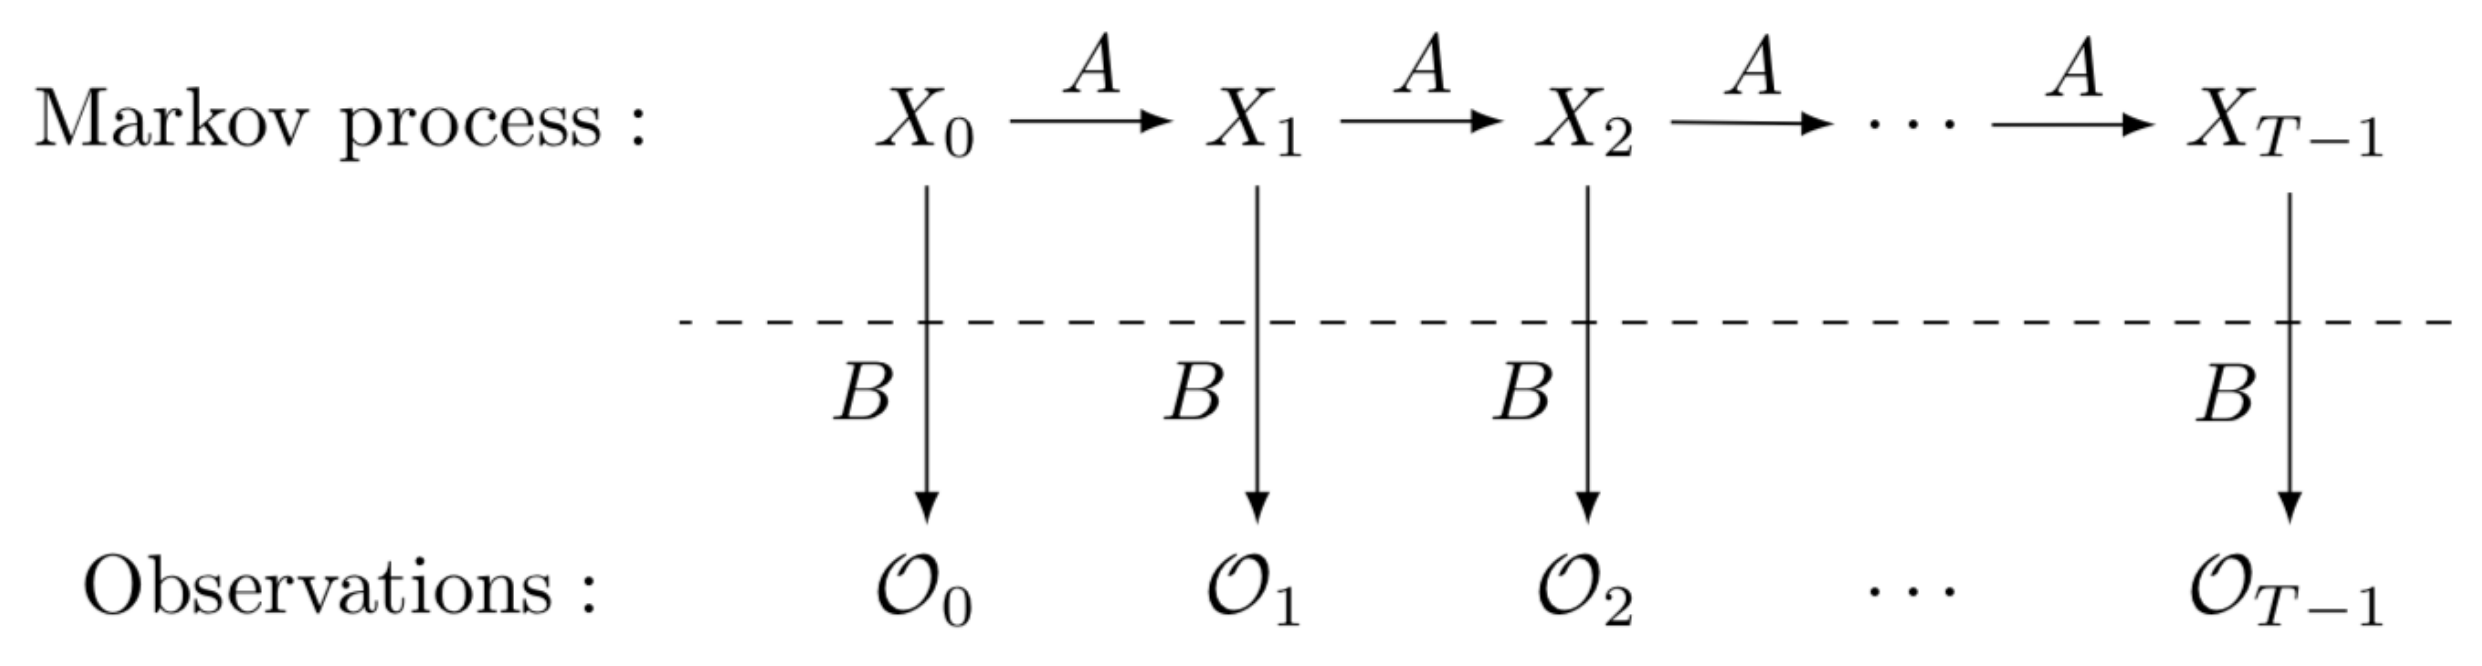
\includegraphics[width=1.0\linewidth]{./HMM.png}
\end{center}

A hidden Markov model (HMM) allows us to talk about both observed events (like words that we see in the input) and hidden events (like part-of-speech tags) that we think of as causal factors in our probabilistic model. HMM model $\lambda$ contains transition probability matrix $A$, a set of state variables $X$, a sequence of observations $O$, emission probabilities $B$, and an initial probability distribution over states $\pi$.

We can characterize HMM into 3 fundamental problems;

1) Likelihood: given the model $\lambda$, find likelihood $P(O|\lambda)$ whether the observation $O$ is a probable sequence based on $\lambda$.

2) Decoding: given an observation sequence $O$ and an model $\lambda$, discover the best hidden state sequence $X$.

3) Learning: given an observation sequence $O$ and the set of states in $\lambda$, learn the parameters $A$ and $B$.

\subsection{Forward Algorithm}

\begin{center}
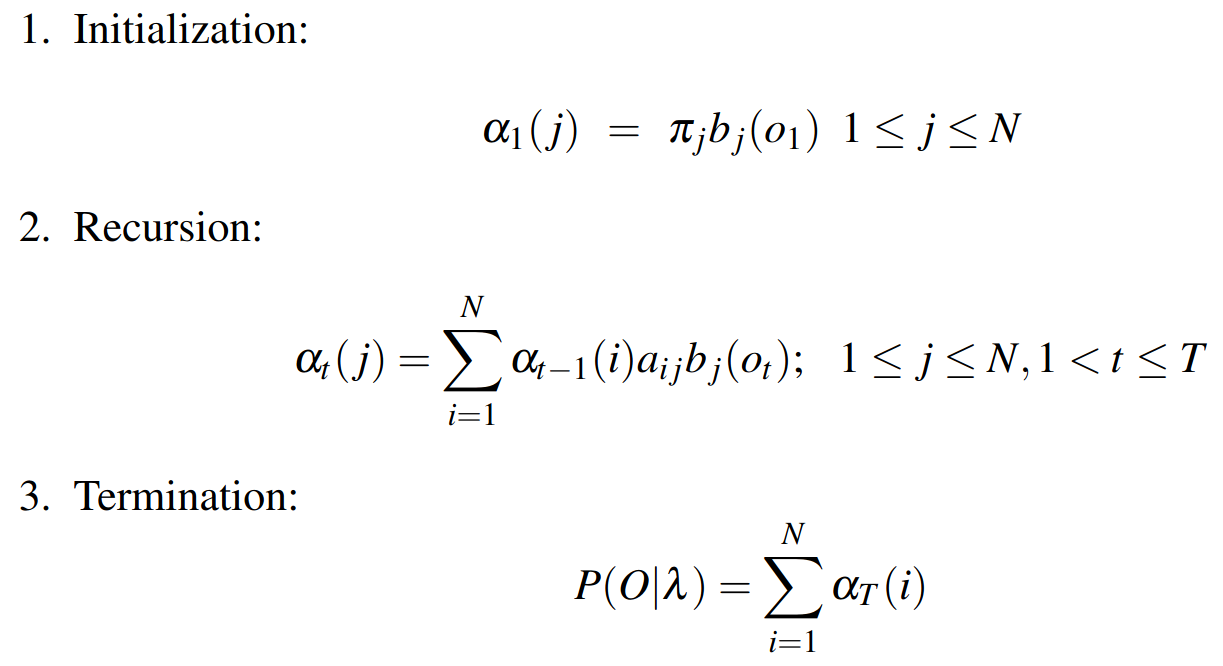
\includegraphics[width=1.0\linewidth]{./forward.png}
\end{center}

We use algorithm called the forward algorithm to compute likelihood of observed events. It is an algorithm that uses a table to store intermediate values as it builds up the probability of the observation sequence. The forward algorithm computes the observation probability by summing over the probabilities of all possible hidden state paths that could generate the observation sequence \cite{hmm}.

\subsection{Baum-Welch Algorithm}
The standard algorithm for HMM training is the forward-backward, or Baum-Welch algorithm, a special case of the Expectation-Maximization algorithm (EM). The algorithm will let us train both the transition probabilities $A$ and the emission probabilities $B$ of model $\lambda$.

%-------------------------------------------------------------------------
\section{Proposed Method}
This section describes overall flows of our proposed method, \texttt{jerk8vel8iter50}. Feature extraction and learning with multinomial HMM are the key concepts of our model.

\subsection{Feature extraction}
Since HAR datasets are given as 3 dimensional vector sets, we have to figure out what feature metric would describe our hidden states of model. We'd like to transform 3 dimensional vectors of acceleration and angular speed into a single metric, so we can train these observations to our HMM model. Figure below shows how we can classify vectors into 8 spaces, A to H, and in number, 0 to 7 \wrt.

\begin{center}
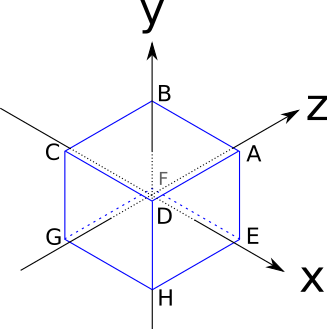
\includegraphics[width=0.5\linewidth]{./coordinate.png}
\end{center}

From acceleration observation data, we can apparently determine the direction of jerk, time derivative of acceleration by subtracting neighbouring values \cite{jerkwiki}.

\begin{center}
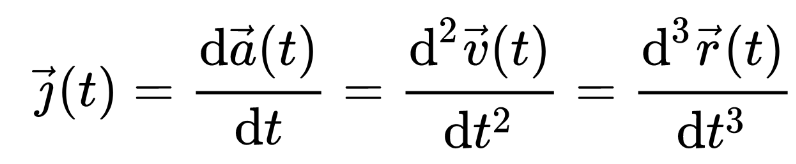
\includegraphics[width=0.6\linewidth]{./jerk.png}
\end{center}

Inferring from the name of our proposed model \texttt{jerk8vel8iter50}, it has 8 jerk states and 8 of those in angular velocity, which is simply determined by signs of vector coordinates. Feature metric is only the measure multiply with these two. For instances, if signs of jerk and angular velocity are $(+,-,+)$ and $(-,-,+)$ each, the measure will be 20 because the state of jerk would be 4(E) and that of angular velocity would be 5(F).

\subsection{Multinomial HMM}
Using model selection package in sklearn \cite{sklearn}, original set was split into train and test data. Every data entity has its feature metric which will be the observation input to HMM model $\lambda$. We differentiated into 12 models by activity types and each model learns corresponding activity and classifies test data set with one vs rest method (OVR) with maximum likelihood. 

As observation values are all in discrete number, Multinomial HMM from \textit{hmmlearn} was selected and values of hyper-parameters were determined through various empirical approaches. We've finally got \texttt{jerk8vel8iter50} model with 00.00\% test accuracy and 00000s total training time. Figures below show a table of 12 models' training time, and some of examples when estimates went wrong.

%-------------------------------------------------------------------------
\section{Empirical Analysis}

Here we describes how we came up with \texttt{jerk8vel8iter50} model. 

\subsection{Feature Metric Approach}
When deciding what feature metric would be suitable, we've compared many different models trained for 1 iteration and chose the metric of the model with best test accuracy.

\subsection{Iteration Approach}

%-------------------------------------------------------------------------
\section{Conclusion}


\begin{thebibliography}{9}

\bibitem{ratgo} 
ratgo’s blog

\bibitem{hmmwiki} 
Wikipedia, Hidden Markov model

\bibitem{biology} 
Byung-Jun Yoon, 
``Hidden Markov Models and their Applications in Biological Sequence Analysis"

\bibitem{speechrecognition} 
M. Gales and S. Young
``The Application of Hidden Markov Models in Speech Recognition".
{\textit{Foundations and Trends in Signal Processing, Vol.1, No.3}, 2007}

\bibitem{hapt}
Jorge L. Reyes-Ortiz, Davide Anguita, Alessandro Ghio, Luca Oneto and Xavier Parra,
``Smartphone-Based Recognition of Human Activities and Postural Transitions Data Set"
, 2015

\bibitem{haptpaper}
Jorge L, \etal
``Human Activity Recognition on Smartphones with Awareness of Basic Activities and Postural Transitions"
{\textit{ICANN 2014, LNCS 8681, pp.177–185}, 2014}

\bibitem{monitoring}
Rubén San-Segundo, Julián David Echeverry-Correa, Christian Salamea, José Manuel Pardo
``Human activity monitoring based on hidden Markov models using a smartphone"
{\textit{IEEE Instrumentation and Measurement Magazine}, 2016}

\bibitem{hmm}
Daniel Jurafsky and James H. Martin.
``Hidden Markov Models"
{\textit{Speech and Language Processing}, 2019}

\bibitem{jerkwiki} 
Wikipedia, Jerk (physics)

\bibitem{sklearn} 
API Documentation of sklearn, model selection, train test split


\end{thebibliography}
% [8] API Documentation of hmmlearn.MultinomialHMM (https://hmmlearn.readthedocs.io/en/latest/api.html#multinomialhmm)

\end{document}
